\documentclass[margin=0px]{article}

\usepackage{listings}
\usepackage[utf8]{inputenc}
\usepackage{graphicx}
\usepackage{float}
\usepackage[a4paper, margin=1in]{geometry}
\usepackage{amsthm}

\renewcommand{\figurename}{ábra}
\newenvironment{tetel}[1]{\paragraph{#1 \\}}{}

\usepackage{listings}
\usepackage{color}



% A dokument itt kezdődik

\title{Záróvizsga tételsor \\ \large 9. Programok fordítása és végrehajtása}
\date{}
\author{}

\begin{document}
	\maketitle
	
	\begin{tetel}{ Programok fordítása és végrehajtása }
		Fordítás és interpretálás összehasonlítása. 
		Fordítási egység és a szerkesztés fogalma.
		Fordítóprogramok komponenseinek feladata és működési elveik vázlatos ismertetése.
		Kódgenerálás assemblyben alapvető imperatív vezérlési szerkezetekhez. 
		A szekvenciális és
		párhuzamos/elosztott végrehajtás összehasonlítása
	\end{tetel}
	
\section{Bevezetés}
	
	
	Amikor programot írunk, azt valamilyen programozási nyelven tesszük. Ezután a nyelvtől függően vagy lefordítjuk, vagy interpreterrel futtatjuk.
	
\section{Fordítás és Interpretálás}
	
\subsection{Fordítás}
	
	A fordítás során általában egy magas szintű programozási nyelvből gépi kód keletkezik, amelyet a processzor már képes értelmezni és futtatni. Előnye, hogy gyors, mivel a lexikális, szintaktikus és szemantikus elemzés fordítási időben, egyszer fut le, valamint ekkor optimalizáljuk a kódot. Fordítási időben sok hibát ki lehet szűrni, ezáltal megkönnyítve a debugolást. A gépi kód nehezen visszafejthető. Általában nagyobb programokhoz használjuk, ahol fontos a hatékonyság. A lefordított kódon később már nem (vagy csak nagyon nehezen) tudunk változtatni.
	
	Hátránya, hogy a keletkezett kód nem platformfüggetlen, minden architektúrára külön-külön le kell fordítani.
	
	\textbf{Példák}: C, C++, Ada, Haskell
	
	\begin{figure}[H]
		\centering
		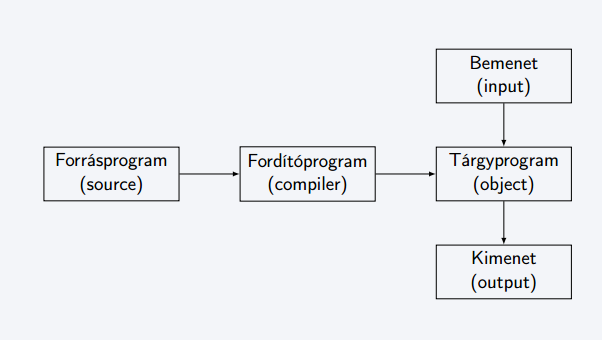
\includegraphics[width=0.5\textwidth]{img/forditas_folyamatabra.png}
		\caption{a fordítás folyamata}
		\label{fig:forditas_folyamatabra}
	\end{figure}
	
	
\subsection{Interpretálás}
	
	Az interpretálás során a programkódot az értelmező futás közben hajtja végre. Platformfüggetlen, csak az interpretert kell minden rendszerre egyszer megírni. Nehéz benne a hibakeresés, mivel sok olyan hiba maradhat a kódban, amit egy fordító kiszűrt volna (pl. típus egyezőség).
	
	\textbf{Példák}: PHP, JavaScript, ShellScript
	

	\begin{figure}[H]
		\centering
		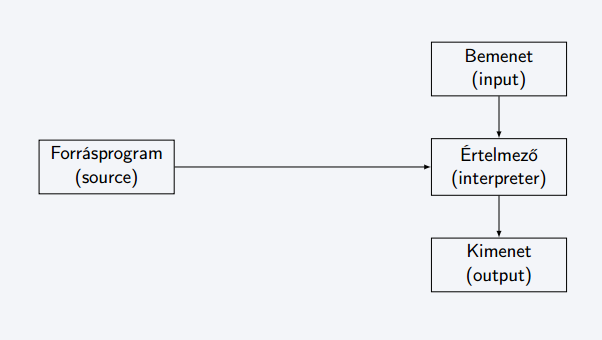
\includegraphics[width=0.5\textwidth]{img/interpretalas_folyamatabra.png}
		\caption{az interpretálás folyamata}
		\label{fig:interpretalas_folyamatabra}
	\end{figure}
	
	
\subsection{Fordítás és Interpretálás együtt}
		
	Egyes nyelvek (pl. Java) előfordítást használnak, melynek eredménye a \textit{bájtkód}, amely gépi kód egy virtuális gép számára. Ezzel elérhető a fordítási idejű hibaellenőrzés és optimalizálás, de megmarad a platformfüggetlenség.
	
	\begin{figure}[H]
		\centering
		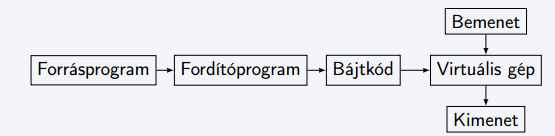
\includegraphics[width=0.5\textwidth]{img/bajtkod_folyamatabra.png}
		\caption{az interpretálás folyamata}
		\label{fig:bajtkod_folyamatabra}
	\end{figure}
	
\section{Fordítási egység és a szerkesztés}
	
	A tárgykód létrehozása két fázisban történik. Először a forrásfájlokat \textit{lefordítjuk}, ebből keletkezik az un. \textit{objektumkód} (pl.: .obj, .class). Ebben a gépi utasítások már megvannak, de hiányzik belőle a hivatkozások (pl változók, függvények), melyek más fájlokban vannak megvalósítva. \textit{Fordítási egységnek} nevezzük azt, amiből egy objektumkód keletkezik.
	
	 A \textit{linker} (szerkesztő) feladata, hogy a hiányzó referenciákat kitöltse, hogy egyetlen fájlt generálva futtatható kódot kapjunk.
	
	 A linkelés lehet statikus, amikor a fordító tölti fel a hiányzó referenciákat; vagy dinamikus, mikor fordítási időben, jellemzően egy másik fájlból (pl.: .dll) tölti be a hiányzó kódot. Az utóbbi akkor praktikus, ha egy modult több, különálló program használ.
	

\section{A fordítóprogram komponensei}	
	\begin{figure}[H]
		\centering
		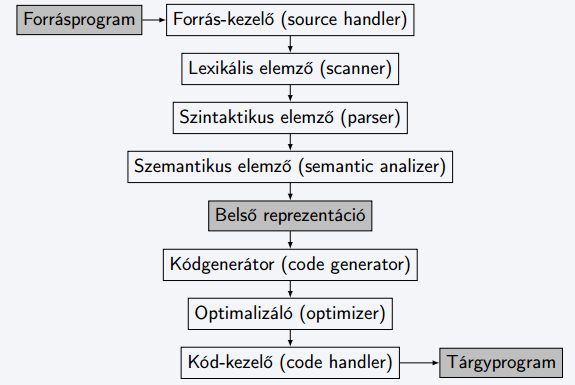
\includegraphics[width=0.5\textwidth]{img/forditas_teljes_folyamata.png}
		\caption{a fordítás lépései}
		\label{fig:forditas_teljes_folyamatabra}
	\end{figure}


\subsection{Lexikális elemző}
	
	Bemenete maga a forráskód. A lexikális elemző feladata, hogy tokenekre bontsa a forráskódot. Adott egy reguláris (hármas típusú) nyelvtan, mely a nyelvre jellemző. Ez adja meg,  hogy milyen típusú tokenek szerepelhetnek a forrásban. A tokenekhez tulajdonságokat rendelhet (pl. változó neve, literál értéke). Kimenete ez a tokensorozat. Amennyiben az elemző olyan karaktersorozatot talál, amelynek nem feleltethető meg token, akkor az lexikális hibát vált ki.
	
	\textit{megjegyzés: Lexikális hibánál nem feltétlen szakad meg a fordítás folyamata, megpróbálhatjuk átugrani az adott részt és folytatni az elemzést, így ha több hiba is van, akkor azokat egyszerre jelezhetjük.}
	
	A reguláris kifejezéseket \textit{véges determinisztikus automatákkal} ismerjük fel. Amennyiben egy lexikális elemre az egyik automata elfogadó állapotba kerül, úgy felismertünk egy tokent. Egy karaktersorozatot egyszerre több automata is felismerhet. Amennyiben ezek azonosan hosszúak, akkor a nyelv konfliktusos. Ennek nem szabad előfordulnia. Az viszont lehetséges, hogy egy szót, és az ő prefixét is felismerte egy automata. Ekkor mindig a hosszabbat választjuk. 
	
\subsection{Szintaktikus elemző}

	Bemenete a lexikális elemző kimenete. Feladata, hogy \textit{szintaxisfát} építsen a tokenekből, a nyelvez tartozó egy környezetfüggetlen (kettes típusú) grammatika alapján, vagy ha ez lehetetlen, akkor jelezze ezt \textit{szintaktikus hiba}ként.
	
\subsubsection{LR0 elemzés}
	
	A lexikális elemző által előállított szimbólumsorozatot balról
	jobbra olvassuk, a szimbólumokat az elemző vermébe tesszük.
	
	\textit{Léptetés}: egy új szimbólumot teszünk a bemenetről a verem
	tetejére.
	
	\textit{Redukálás}: a verem tetején lévő szabály-jobboldalt
	helyettesítjük a szabály bal oldalán álló nemterminálissal
	
	A háttérben egy véges determinisztikus automata működik:
	az automata átmeneteit a verem tetejére kerülő szimbólumok
	határozzák meg
	ha az automata végállapotba jut, redukálni kell
	egyéb állapotban pedig léptetni.
	
	Az automata bizonyos nyelvek esetén konfliktusos lehet: nem tudjuk eldönteni, hogy léptessünk vagy redukáljunk.
	
\subsubsection{LR1 elemzés}
	
	Az előző problémára kínál megoldást, kibővítve a lehetséges nyelvek halmazát.
	
	Az ötlet, hogy \textit{olvassunk előre} egy szimbólumot.
	
	Ha az aktuális állapot \textit{i}, és az előreolvasás eredménye az a
	szimbólum:
	
	ha $ [A	\rightarrow \alpha.a\beta, b] \in I_i $ és $read(I_i, a) = I_j$
	akkor léptetni kell, és átlépni a \textit{j} állapotba.
	
	
	ha $ [A	\rightarrow \alpha., a] \in I_i (A \neq S'), $
	akkor redukálni kell az $ A \rightarrow \alpha $ szabály szerint.
	
	
	
	
	ha $ [S' \rightarrow S., \#] \in I_i $ és $ a = \# $, akkor el kell fogadni a szöveget,	minden más esetben hibát kell jelezni.
	
	Ha az \textit{i} állapotban \textit{A} kerül a verem tetejére:
		ha$  read(I_i,A) =	I_j $ , 
	akkor át kell lépni a \textit{j} állapotba,	egyébként hibát kell jelezni.

	
	 
\subsubsection{Jelmagyarázat/Kanonikus halmazok}
	
	\paragraph{Closure/lezárás}
	
	Ha $ I $ a grammatika egy $ LR(1) $ elemhalmaza, akkor $ closure(I) $ a
	legszűkebb olyan halmaz, amely az alábbi tulajdonságokkal
	rendelkezik:
	
	$ I \subseteq closure(I) $ ha $ [A \rightarrow \alpha.B\gamma,a] \in closure(I) $, 
	
	és $ B \rightarrow \beta $ a grammatika egy szabálya,
	 akkor $ \forall b \in FIRST1(\gamma{}a) $ esetén $ [B \rightarrow .\beta,b] \in closure(I) $
	
	
	\paragraph{Read/olvasás}
	Ha $ I $ a grammatika egy $ LR(1) $ elemhalmaza, $ X $ pedig terminális	vagy nemterminális szimbóluma, akkor $ read(I, X) $ a legszűkebb olyan halmaz, amely az alábbi tulajdonsággal rendelkezik:
	
	Ha $ [A \rightarrow \alpha. X\beta,a] \in I $, akkor $ closure([ A \rightarrow \alpha X.\beta,a]) \subseteq read(I, X) $. 
	
	
	\paragraph{LR(1) kanonikus halmazok ($ I_n $)}
	\begin{itemize}
		\item 
		$ closure([S' \rightarrow .S, \#]) $ a grammatika egy kanonikus halmaza.
		\item 
		Ha $ I $ a grammatika egy kanonikus elemhalmaza, $ X $ egy terminális vagy nemterminális szimbóluma, és $ read(I, X) $ nem üres, akkor $ read(I, X) $ is a grammatika egy kanonikus halmaza.
		\item 
		Az első két szabállyal az összes kanonikus halmaz előáll.
	\end{itemize}
		
	
	
	
\subsection{Szemantikus elemző}
	

	A szemantikus elemzés jellemzően a környezetfüggő ellenőrzéseket
	valósítja meg.
	
	%Dévai diáiról
	\begin{itemize}
		\item 
		deklarációk kezelése: változók, függvények, eljárások, operátorok, 	típusok
		\item
		láthatósági szabályok
		\item
			aritmetikai ellenőrzések
		\item
		a program szintaxisának környezetfüggő részei
		\item 
		típusellenőrzés
		\item 
		stb. 
	\end{itemize}
	
	
	A szemantikus elemzéshez ki kell egészítenünk a grammatikát. Rendeljünk a szimbólumokhoz attribútumokat és a szabályokhoz akciókat! Egy adott szabályhoz tartozó feltételek csak a szabályban	előforduló attribútumoktól függhetnek.	(Ha egy feltétel nem teljesül, akkor szemantikus hibát kell	jelezni!). A szemantikus rutinok csak annak a szabálynak az	attribútumait használhatják és számíthatják ki, amelyikhez az őket reprezentáló akciószimbólum tartozik. Minden szintaxisfában minden attribútumértéket pontosan egy
	szemantikus rutin határozhat meg. Az így létrejövő nyelvtant \textit{attribútum fordítási grammatikának} (ATG) hívjuk.

	A \textit{jól definiált attribútum fordítási grammatika}, olyan attribútum fordítási grammatika, amelyre igaz, hogy a	grammatika által definiált nyelv mondataihoz tartozó minden szintaxisfában minden attribútum értéke egyértelműen kiszámítható.
	
	Egy attribútumot kétféleképpen lehet meghatározni:
	
	\paragraph{Szintézissel} a szintaxisfában alulról felfelé terjed az információ, egy szülő attribútumát a gyerekekből számoljuk. Kitüntetettnek hívjuk azokat az attribútumokat, melyeket a lexikális elemző szolgáltat.
	
	\paragraph{Öröklődéssel} a szintaxisfában felülről lefelé terjed az információ. A gyerekek attribútumait a szülőé határozza meg.
	
	Az \textit{L-ATG} olyan attribútum fordítási grammatika, amelyben minden
	$ A	\rightarrow	X_1X_2 . . .	X_n  $szabályban az attribútumértékek az alábbi sorrendben meghatározhatók:
	
	\begin{itemize}
		\item 
		A örökölt attribútumai
		\item 
		$ X_1 $ örökölt attribútumai
		\item 
		$ X_1 $ szintetizált attribútumai
		\item 
		$ X_2 $ örökölt attribútumai
		\item 
		$ X_2 $ szintetizált attribútumai
		\item 
		\dots
		\item 
		$ X_n $ örökölt attribútumai
		\item 
		$ X_n $ szintetizált attribútumai
		\item 
		A szintetizált attribútumai
	\end{itemize}

	Amennyiben a nyelvtanunk ennek eleget tesz, úgy hatékonyan meghatározható minden attribútum.

	A szemantikus elemzéshez jellemzően szimbólumtáblát használunk, verem szerkezettel és keresőfával vagy hash-táblával. Minden blokk egy új szint a veremben, egy szimbólum keresése a verem tetejéről indul.
	
	
	
	
% Kódgenerálás assemblyben alapvető imperatív vezérlési szerkezetekhez. 
\section{Kódgenerálás alapvető vezérlési szerkezetekhez}


	A kódgenerálás feladata, hogy a szintaktikusan és szemantikusan elemzett programot tárgykóddá alakítsa. Általában szorosan összekapcsolódik a
	szemantikus elemzéssel. 
	
\subsection{Értékadás}
	
	assignment $ \rightarrow $ variable assignmentOperator expression

	\begin{verbatim}
		a kifejezést az eax regiszterbe kiértékelö kód
		2 mov [Változó],eax
	\end{verbatim}
	
\subsection{Egy ágú elágazás}
	statement $ \rightarrow $ if condition then program end
	
	\begin{verbatim}
		1 a feltételt az al regiszterbe kiértékelö kód
		2 cmp al,1
		3 je Then
		4 jmp Vége
		5 Then: a then-ág programjának kódja
		6 Vége:
	\end{verbatim}
	
	\textit{megjegyzés: a dupla ugrásra azért van szükség, mert a feltételes ugrás hatóköre limitált.}

\subsection{Több ágú elágazás}

	
	statement $ \rightarrow $ 
	\\if $ condition_1 $ then $ program_1 $ 
	\\elseif $ condition_2 $ then $ program_2 $ 
	\\\dots
	\\elseif $ condition_n $ then $ program_n $
	\\else $ program_{n+1} $ end
	
	\begin{verbatim}
		1 az 1. feltétel kiértékelése az al regiszterbe
		2 cmp al,1
		3 jne near Feltétel_2
		4 az 1. ág programjának kódja
		5 jmp Vége
		6
		...
		7 Feltétel_n: az n-edik feltétel kiértékelése az al regiszterbe
		8 cmp al,1
		9 jne near Else
		10 az n-edik ág programjának kódja
		11 jmp Vége
		12 Else: az else ág programjának kódja
		13 Vége:
	\end{verbatim}

\subsection{Switch-case}
	statement $ \rightarrow $ switch variable
	\\case $ value_1 $ : $ program_1 $
	\\...
	\\case $ value_n $ : $ program_n $
	
	\begin{verbatim}
		1 cmp [Változó],Érték_1
		2 je near Program_1
		3 cmp [Változó],Érték_2
		4 je near Program_2
		5
		. ..
		6 cmp [Változó],Érték_n
		7 je near Program_n
		8 jmp Vége
		9 Program_1: az 1. ág programjának kódja
		10
		. ..
		11 Program_n: az n-edik ág programjának kódja
		12 Vége:
	\end{verbatim}

\subsection{Ciklus}
%Ez egy vagy két szó?
\subsubsection{Elől tesztelő}	
	statement $ \rightarrow $ while condition statements end
	
	\begin{verbatim}
		1 Eleje: a ciklusfeltétel kiértékelése az al regiszterbe
		2 cmp al,1
		3 jne near Vége
		4 a ciklusmag programjának kódja
		5 jmp Eleje
		6 Vége:
	\end{verbatim}
	
	
%Ez egy vagy két szó?
\subsubsection{Hátul tesztelő}	
	statement $ \rightarrow $ loop statements while condition


	\begin{verbatim}
		1 Eleje: a ciklusmag programjának kódja
		2 a ciklusfeltétel kiértékelése az al regiszterbe
		3 cmp al,1
		4 je near Eleje
	\end{verbatim}
	
\subsubsection{For ciklus}	

	statement $ \rightarrow $ for variable from $ value_1 $ to $ value_2 $ statements end
	
	
	\begin{verbatim}
		1 a "from" érték kiszámítása a [Változó] memóriahelyre
		2 Eleje: a "to" érték kiszámítása az eax regiszterbe
		3 cmp [Változó],eax
		4 ja near Vége
		5 a ciklusmag kódja
		6 inc [Változó]
		7 jmp Eleje
		8 Vége:
	\end{verbatim}

\subsection{Statikus változók}
	
	Kezdőérték nélküli változódefiníció fordítása:
	\begin{verbatim}
		section .bss
		; a korábban definiált változók...
		Lab12: resd 1 ; 1 x 4 bájtnyi terület
	\end{verbatim}

	
	Kezdőértékkel adott változódefiníció fordítása:
	\begin{verbatim}
		section .data
		; a korábban definiált változók...
		Lab12: dd 5 ; 4 bájton tárolva az 5-ös érték
	\end{verbatim}

\subsection{Logikai kifejezések}

\subsubsection{kifejezés1 $ < $  kifejezés2 }
	
	\begin{verbatim}
		; a 2. kifejezés kiértékelése az eax regiszterbe
		push eax
		; az 1. kifejezés kiértékelése az eax regiszterbe
		pop ebx
		cmp eax,ebx
		jb Kisebb
		mov al,0 ; hamis
		jmp Vége
		Kisebb:
		mov al,1 ; igaz
		Vége:
	\end{verbatim}

\subsubsection{kifejezés1 $ \lbrace $ és, vagy, nem, kizáróvagy  $ \rbrace $  kifejezés2 }

	\begin{verbatim}
		; a 2. kifejezés kiértékelése az al regiszterbe
		push ax ; nem lehet 1 bájtot a verembe tenni!
		; az 1. kifejezés kiértékelése az al regiszterbe
		pop bx ; bx-nek a bl részében van,
		; ami nekünk fontos
		and al,bl
	\end{verbatim}
	
\subsubsection{ lusta "és" kiértékelés }
	
	\begin{verbatim}
		; az 1. kifejezés kiértékelése az al regiszterbe
		cmp al,0
		je Vége
		push ax
		; a 2. kifejezés kiértékelése az al regiszterbe
		mov bl,al
		pop ax
		and al,bl
		Vége:
	\end{verbatim}
	

\subsubsection{ Alprogramok megvalósítása }
	
	
	\begin{verbatim}
		; az 1. kifejezés kiértékelése az al regiszterbe
		cmp al,0
		je Vége
		push ax
		; a 2. kifejezés kiértékelése az al regiszterbe
		mov bl,al
		pop ax
		and al,bl
		Vége:
	\end{verbatim}
	
\subsubsection{ Alprogramok hívása }

	\begin{verbatim}
		Alprogramok sémája
		; utolsó paraméter kiértékelése eax-be
		push eax
		; ...
		; 1. paraméter kiértékelése eax-be
		push eax
		call alprogram
		add esp,’a paraméterek összhossza’
	\end{verbatim}
	
\section{Kódoptimalizáló}
	
	Az optimalizálás feladata, hogy a keletkezett kód kisebb és gyorsabb legyen, úgy hogy a futás eredménye nem változik. A gyorsaság és a tömörség gyakran ellentmondanak egymásnak, és az egyik csak a másik rovására lehet javítani. Általában három lépésben szokás elvégezni:
	
	\begin{itemize}
		\item 
		Optimalizálási lépések végrehajtása az eredeti programon (vagy annak egyszerűsített változatán)
		\item 
		Kódgenerálás
		\item 
		Gépfüggő optimalizálás végrehajtása a generált kódon
	\end{itemize}
	
\subsection{Lokális optimalizáció} 
	
	Egy programban egymást követő utasítások sorozatát \textit{alapblokknak} nevezzük, ha az első utasítás kivételével egyik utasítására sem lehet távolról átadni a vezérlést (assembly programokban: ahová a jmp, call, ret utasítások "ugranak"; magas szintű nyelvekben: eljárások, ciklusok eleje, elágazások ágainak első utasítása, goto utasítások célpontjai). Az utolsó utasítás kivételével nincs benne vezérlés-átadó utasítás (assembly programban: jmp, call, ret magas szintű nyelvekben: elágazás vége, ciklus vége, eljárás vége, goto). Az utasítás-sorozat nem bővíthető a fenti két szabály megsértése nélkül.
	
	Ha az optimalizálás az alapblokkok keretein belül történik, akkor garantált, hogy az átalakításnak nincs mellékhatása. Ez a \textit{lokális optimalizálás}.
	
	\paragraph{Ablakoptimalizálás}
	Ez egy módszer a lokális optimalizálás egyes fajtáihoz. Egyszerre csak egy néhány utasításnyi részt vizsgálunk a kódból. A vizsgált részt előre megadott mintákkal hasonlítjuk össze. Ha illeszkedik, akkor a mintához megadott szabály szerint átalakítjuk ezt az "ablakot" végigcsúsztatjuk a programon. Az átalakítások megadása:
	\begin{center}
	$ \lbrace$ minta $ \rightarrow $ helyettesítés $\rbrace$ szabályhalmazzal
	(a mintában lehet paramétereket is használni)
	\end{center}

	Példák:
	\begin{itemize}
		\item 
		felesleges műveletek törlése: nulla hozzáadása vagy kivonása
		\item 
		egyszerűsítések: nullával szorzás helyett a regiszter törlése
		\item 
		regiszterbe töltés és ugyanoda visszaírás esetén a visszaírás elhagyható
		\item 
		utasításismétlések törlése: ha lehetséges, az ismétlések törlése
	\end{itemize}
	

\subsection{Globális optimalizáció} 
	A teljes program szerkezetét meg kell vizsgálni. Ennek módszere az adatáram-analízis:
	\begin{itemize}
		\item 
		Mely változók értékeit számolja ki egy adott alapblokk?
		\item 
		Mely változók értékeit melyik alapblokk használja fel?
	\end{itemize}
	
	
	Ez lehetővé teszi az azonos kifejezések többszöri kiszámításának kiküszöbölését akkor is, ha különböző alapblokkokban szerepelnek; valamint a konstansok és változók továbbterjesztését alapblokkok között is elágazások, ciklusok optimalizálását.

	% kell ide példa? tudok szerezni de nem hiszem hogy annyira fontos lenne
	
\section{A szekvenciális és	párhuzamos/elosztott végrehajtás összehasonlítása}
	
\subsection{Szekvenciális végrehajtás:}

	Ilyenkor a végrehajtás egy processzoron történik. Minden művelet atomi. Egy inputhoz egy output tartozik. Két szekvenciális program ekvivalens, ha ezek a párosok megegyeznek. Nem használja fel az összes rendelkezésre álló erőforrást.


\subsection{Párhuzamos végrehajtás:}		
	
	Több processzoron hajtódik végre a program. A párhuzamos folyamatok egymással kommunikálva, szinkronban oldják meg az adott problémát. A konkurens program szétbontható elemi szekvenciális programokra, ezek a folyamatok. A folyamatok használhatnak közös erőforrásokat: pl. változók, adattípus  objektumok, kommunikációs csatornák.
	
	A kommunikációt általában kétféleképpen szokták megvalósítani.
	\paragraph{Osztott memóriával.} Ekkor szinkronizálni kell, hogy ki mikor fér hozzá, hogy ne legyen ütközés.

	\paragraph{Kommunikációs csatornával.} Garantálni kell, hogy ha egy folyamat üzenetet küld egy másiknak, akkor az meg is kapja azt, és jelezzen is vissza. Ügyelni kell, nehogy deadlock alakuljon ki.
		
\end{document}



